% http://cds.cern.ch/record/2804003?ln=en
% see citation of the PAS from CV 

In addition to analyzing data already taken by the CMS detector during LHC Run 2, and further developing the detector's data-taking features to improve physics sensitivity during LHC Run 3, it is important to perform projection studies in order to estimate the expected sensitivity to physics processes with future particle accelerators and upgraded detectors. These studies provide physicists with initial insight of what to expect when performing future measurements and searches, and can motivate which analyses to perform in the future.

Through the results of the search for di-Higgs production in the WW$\gamma\gamma$ final state using the LHC Run 2 dataset, it is difficult to obtain an accurate estimate of the analysis sensitivity at the future HL-LHC with the upgraded CMS detector. In order to perform this projection, a separate simulation-only analysis is performed. In addition, the \ttgg HH final state is added to this search as it has a similar final state topology to \wwgg. 

The structure of this chapter is as follows: The strategy of the analysis will be described in Section \ref{sec:Strategy_Phase_II}. The phase II CMS detector will be described in Section \ref{section:Phase_II_CMS}. The simulated samples used in this analysis will be described in Section \ref{sec:Phase_II_Samples}. Object selection is described in Section \ref{sec:Phase_II_ObjectSel}. Event selection and categorization will be described in Section \ref{sec:Phase_II_Selections}. A description of the systematic uncertainties considered is described in Section \ref{sec:Phase_II_Systematics}. The results of the analysis are presented in Section \ref{sec:Phase_II_results}, and the analysis is summarized in Section \ref{sec:Phase_II_Summary}. 

\section{Strategy} \label{sec:Strategy_Phase_II}

For the \wwgg portion of this analysis, the strategy is very similar to that of the Run 2 analysis. For the \ttgg portion of the analysis, a similar analysis strategy is followed with respect to the semi-leptonic final state of the Run 2 analysis, namely through the use of a DNN. 

For both HH final states, the signal and background topologies are the same as for the Run 2 analysis as the upgrade in the LHC and CMS detector will not dramatically change the signal and background signatures. In this analysis, a simulation template is formed for HH, H and a continuum of background process. As there is not yet a Phase II dataset to use for a statistical interpretation via a fitting of the simulation templates to the data, a projection is made by fitting the background-only hypothesis simulation templates to the signal $+$ background simulation templates in order to estimate how clear of an HH signature is expected to be seen in the Phase II CMS dataset. This is performed in a signal region defined as the diphoton invariant mass, in the window 115 $<$ $\mgg$ $<$ 135. This region is chosen due to the expectation that the H$\rightarrow\gamma\gamma$ leg of the HH$\rightarrow$(WW$+\tau\tau$) $\gamma\gamma$ processes should provide a peak in this region. 

As was the case for the Run 2 analysis, there are two background signatures present in this analysis: A resonant background from the single Higgs to $\gamma\gamma$ process, and a continuum background formed by a combination of background processes which do not contain a prompt diphoton. An illustration of signal and background signatures is shown in Figure \ref{fig:Signatures}.

In order to optimize the sensitivity of this analysis,
a DNN (Deep Neural Network) is employed for the Semi-Leptonic WW$\gamma\gamma$ final state and one Tau \ttgg final state. These final states are expected to be the most sensitive due to the increase in branching ratio
from their hadronic decays, but with the benefit of maintaining a clean signature due to the presence of a lepton in their leptonic decays.

For the Fully-Leptonic \wwgg and two Tau \ttgg channels, cut based strategies are performed due to a lack of number of events.

In order to combine all final state categories in order to extract a more sensitive final result, it is imperative to apply orthogonal selections to simulation events in order to avoid including the same events in multiple background categories. This is done via the event's number of leptons, namely the number of electrons and muons in the \wwgg categories, and number of $\tau$ particles in the \ttgg categories. Each lepton must pass a common set of selections applied for all final state tags. After a set of lepton objects is selected for each simulation event, events fall into the Semi-leptonic \wwgg category if they contain exactly one lepton, the Fully-leptonic \wwgg category if they contain at least two leptons, and the one (two) $\tau$ \ttgg category if they contain exactly one (two) hadronically decaying $\tau$ particles. 

Further event selections are made for the each final state category,
but by requiring an orthogonal separation of the number of electrons, muons and $\tau$ particles, it is guaranteed no one event can fall into more than one category. Thus, background and signal models
in different final state categories can be simultaneously fit to pseudo-data in order to obtain a final result which benefits from a combination of the physics signatures of all final states. 

\section{The Phase-2 CMS detector}
\label{section:Phase_II_CMS}

The CMS detector~\cite{Chatrchyan:2008aa} will be substantially upgraded in order to fully exploit the physics potential offered by the increase in luminosity, and to cope with the demanding operational conditions at the HL-LHC~\cite{CMSCollaboration:2015zni, Klein:2017nke, Collaboration:2283187, Collaboration:2293646, Collaboration:2283189}. The upgrade of the first level hardware trigger (L1) will allow for an increase of L1 rate and latency to about 750\unit{kHz} and 12.5\mus, respectively, and the high-level software trigger (HLT) is expected to reduce the rate by about a factor of 100 to 7.5\unit{kHz}. The entire pixel and strip tracker detectors will be replaced to increase the granularity, reduce the material budget in the tracking volume, improve the radiation hardness, and extend the geometrical coverage and provide efficient tracking up to pseudorapidities of about $|\eta|=4$. The muon system will be enhanced by upgrading the electronics of the existing cathode strip chambers (CSC), resistive plate chambers (RPC) and drift tubes (DT). New muon detectors based on improved RPC and gas electron multiplier (GEM) technologies will be installed to add redundancy, increase the geometrical coverage up to about $|\eta|=2.8$, and improve the trigger and reconstruction performance in the forward region. The barrel electromagnetic calorimeter (ECAL) will feature the upgraded front-end electronics that will be able to exploit the information from single crystals at the L1 trigger level, to accommodate trigger latency and bandwidth requirements, and to provide 160\unit{MHz} sampling allowing high precision timing capability for photons. The hadronic calorimeter (HCAL), consisting in the barrel region of brass absorber plates and plastic scintillator layers, will be read out by silicon photomultipliers (SiPMs). The endcap electromagnetic and hadron calorimeters will be replaced with a new combined sampling calorimeter (HGCal) that will provide highly-segmented spatial information in both transverse and longitudinal directions, as well as high-precision timing information. Finally, the addition of a new timing detector for minimum ionizing particles (MTD) in both barrel and endcap regions is envisaged to provide the capability for 4-dimensional reconstruction of interaction vertices that will significantly offset the CMS performance degradation due to high PU rates.

A detailed overview of the CMS detector upgrade program is presented in Ref.~\cite{CMSCollaboration:2015zni, Klein:2017nke, Collaboration:2283187, Collaboration:2293646, Collaboration:2283189, CMS:2667167, CERN-LHCC-2020-004, Collaboration:2759072}, while the expected performance of the reconstruction algorithms and pile-up mitigation with the CMS detector is summarised in Ref.~\cite{Collaboration:2650976}.


\section{Simulated samples} \label{sec:Phase_II_Samples}

Because this analysis is a projection study of the prospects for \wwgg and \ttgg searches as the future HL-LHC and upgraded CMS detector, the samples used in the analysis are exclusively simulation. 

As was done for the Run 2 analysis, signal Monte Carlo $gg\rightarrow HH$ samples are generated using \textsc{Powheg v2} \cite{Nason:2004rx, Frixione:2007vw, Alioli:2010xd, Heinrich:2019bkc} 
at next-to-leading order (NLO) in QCD including the full top quark mass dependence with the SM parameters. 

Subsequent decays of the Higgs boson pairs into WW or $\tau\tau$ and a pair of photons are implemented using \textsc{Pythia 8.212} \cite{Sjostrand:2014zea}. \wwgg samples are generated separately for each final state in \wwgg. 
For \ttgg signal samples, all possible decays for taus are allowed.

As the process signature remains the same for both the Run 2 and Phase II analyses, the expected background signatures also remain the same. The analysis is affected by backgrounds from single Higgs boson production and by non-resonant backgrounds with continuum $m_{\gamma\gamma}$ spectra.
The event generator \textsc{Madgraph5\_amcatnlo} \cite{Alwall:2014hca, Artoisenet:2012st} with the FxFx merging scheme \cite{Frederix:2012ps} was used for the generation of the background from SM single Higgs boson production, including  gluon-gluon fusion (ggH), vector-boson fusion (VBFH), associated production with a Z or W boson (VH)  and associated production with a top quark pair (ttH). The additional single Higgs production mode of top quark associated production (tHq) is also included, and was generated using \textsc{Madgraph} version-2.7 at LO. 

The continuum background contribution comes from various SM processes. Most of the dominant backgrounds
across all the final states are due to the $\gamma\gamma+$jets processes that are 
modeled with the \textsc{Sherpa} v.2.2.1 generator \cite{Bothmann:2019yzt}.
$\gamma+$jets, QCD-induced processes and WW processes are modeled with the PYTHIA 8 \cite{Sjostrand:2014zea} generator.

Drell Yan and W production processes in association with photons and jets are modeled using \textsc{Madgraph5} version-2.7 at LO. 
Finally, the $t\bar{t}$ process is generated using \textsc{Powheg} v2, and $t\bar{t}W$, $t\bar{t}\gamma$, $t\bar{t}\gamma\gamma$, Z$\gamma$ are modeled using \textsc{Madgraph5\_amcatnlo} \cite{Alwall:2014hca,Artoisenet:2012st,Frederix:2012ps}.

For these simulation samples, all are simulated with the Phase-2 upgraded CMS detector geometry using \textsc{Delphes} fast simulation  
with average pile-up of 200 interactions and at 
$\sqrt{s}=14$ TeV, the expected data-taking conditions at the HL-LHC. 
\section{Objects}
\label{sec:Phase_II_ObjectSel}

Before applying final-state specific category selections, a common set of object selections is required for the various physics objects reconstructed event-by-event for each simulation sample. In order to maximize the number HH events saved, each simulation event is required to have at least one pair of photons, called a diphoton.

Photons used in this analysis are required to have a transverse momentum ($p_T$) above 25 GeV, and at least one photon with a \pt of 35 GeV
within $|\eta| < 2.5$.

The relative isolation of the photon
candidate, defined as sum of the $p_T$ of all particles within a cone ($\Delta R = \sqrt{(\Delta \eta)^2 + (\Delta \phi)^2}$) of size 0.3 around the photon and divided the sum by the photon $p_T$, 
is required to be less than 0.3 and must pass a loose identification criteria corresponding to 90\% signal efficiency.

Electrons are required to have $p_T$ above 10 GeV within $|\eta| < 2.5$ excluding the ECAL transition region and 
must be isolated from photon candidates with an angular separation in the $\eta-\phi$ plane greater than $\Delta R = $ 0.4. 
The transverse momenta of muons are required to be above 10 GeV and within $|\eta| < 2.5$ 
, and they are required to be isolated from photon and electron candidates with an angular separation greater than $\Delta R = $ 0.4. 
Hadronically decaying taus are required to have $p_T >$ 20 GeV within $|\eta| < 2.5$, and are required to be separated from photon, electron and muon candidates  
with an angular separation greater than $\Delta R = $0.2. The relative isolation of the electrons (muons) is required to be less than 0.3 (0.1).

Jets are reconstructed using the anti-$k_{T}$ clustering method with a distance parameter of 0.4. 
They are required to have $p_T >$ 30 GeV, be within $|\eta| < 5$ and to be well separated from the photon and lepton candidates with an angular separation greater than $\Delta R = $ 0.4. The likelihood that a jet comes from b-quark hadronization, termed a b-tagging score, is computed using a deep neural network (DNN) based secondary vertex algorithm, \textsc{Deepjet}~\cite{CMS-DP-2018-058, Bols:2020bkb}. 

\section{Event Selections and Categorization}
\label{sec:Phase_II_Selections}  
All events are required to have exactly two photons with an invariant mass in the range $100 < \mgg < 180$\GeV. The analysis is performed in mutually exclusive final states targeting decays of the vector bosons referred to as 1L (Semi-leptonic) and 2L (Fully-leptonic) final states for \wwgg, and 1 $\tau$ or 2 $\tau$ final states for \ttgg. 

Here, lepton (L) refers to either an electron ($e^{\pm}$) or muon ($\mu^{\pm}$). 

\subsection{Semi-leptonic final state}
\label{sec:oneL} 

Events fall into the Semi-leptonic (1L) analysis category if they contain at least one pre-selected diphoton pair, and contain exactly one electron or muon passing the selection criteria described in Section \ref{sec:Phase_II_ObjectSel}. This final state is expected to be the most sensitive of the three $WW\gamma\gamma$ channels due to the combination of a relatively large $W\rightarrow qq$ branching ratio, and the presence of a highly energy lepton from the $W\rightarrow \ell\nu$ decay. 

In order to maximize the sensitivity of this final state, two multiclass DNNs are trained to separate the di-Higgs signal from the resonant single Higgs boson background and continuum background where the di-Higgs processes are labelled as \textit{HH}, single Higgs backgrounds as \textit{H} and all other background samples as continuum background.

% (HH $\rightarrow$ 2$\gamma 2ql\nu$, HH $\rightarrow$ $2\gamma 2\tau$, HH $\rightarrow 2 \gamma 2l2\nu$) 

During training, each class has a weight applied which scales the event loss such that the effective importance's of each of the three classes are equalized. This ensures that the network focuses on categorising all classes with an equal importance. 

Two multiclass DNNs are trained, one which trains on one half of simulation events, and a second which trains on the other half of simulation events. This separation on simulation datasets allows one to apply the training performed with “even” events on the “odd” data set, and vice versa, to avoid any training bias.

The simulation sample variables used as inputs for the DNN trainings include the kinematic variables such as $p_T$, $\eta$, $\phi$ and energy values of photons, jets, electrons and muons. For photons, $p_T$ and energy values are scaled by the diphoton mass in order to avoid the creation of an artificial resonance among continuum background processes. Additionally, the jet multiplicity, missing transverse energy and the invariant mass of the leading and subleading jets are utilized in the trainings. 

The multiclass DNN outputs three DNN scores, one for each class, but only the HH output DNN score is used in the analysis. The HH DNN score distribution is shown in Figure \ref{fig:oneL_perf}. 

\begin{figure}[!htb]
    \centering
    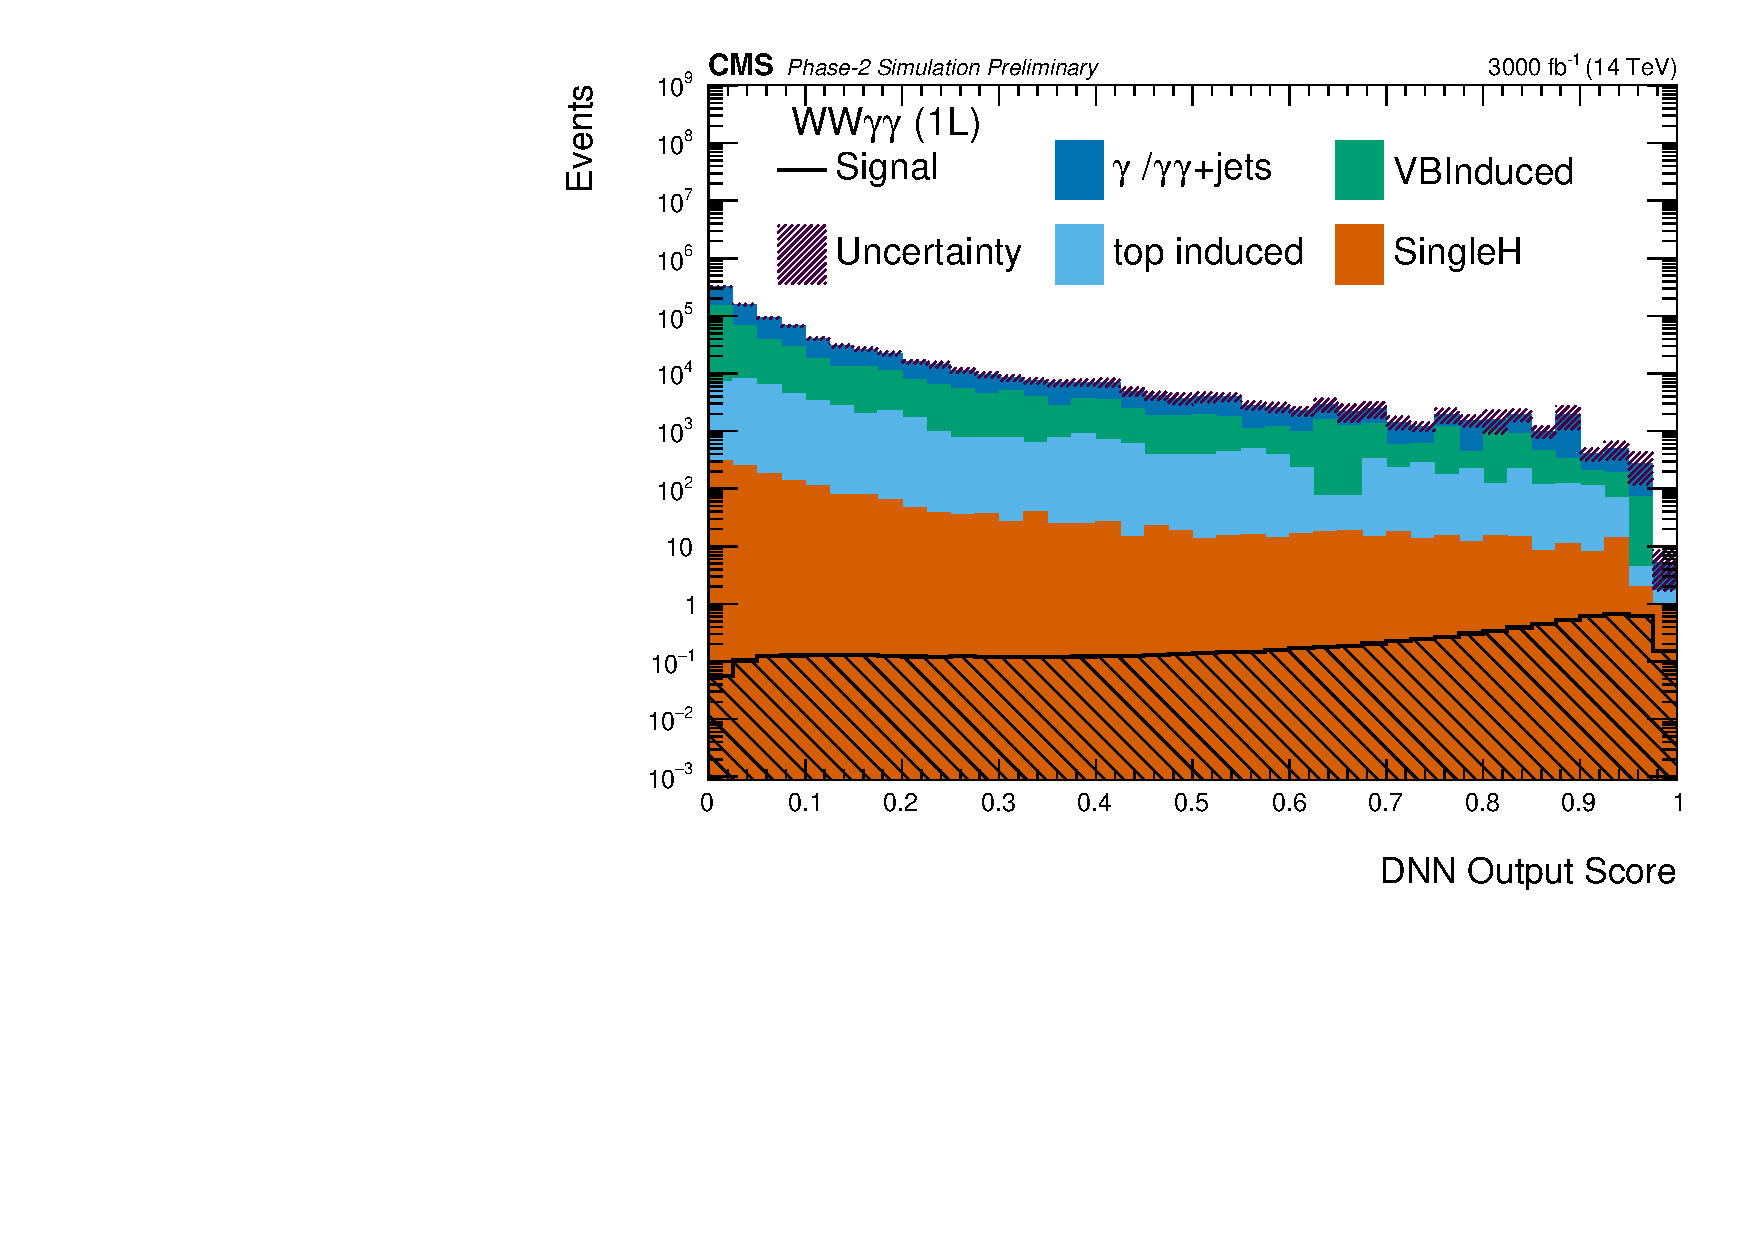
\includegraphics[width=0.75\textwidth]{Sections/Phase_II_HH/images/DNN/DNN_Score_WW_logy.pdf}
    \caption{Semi-leptonic DNN output score distribution.}
    \label{fig:oneL_perf}
\end{figure}

In order to further optimize the analysis sensitivity, events are partitioned into four categories making use of the \textit{HH} node output score. The category boundaries are chosen such that the expected significance is maximized, and are shown in Table \ref{tab:OneLcats}.

\begin{table}[!htb]
  \centering
  \begin{tabular}{ll}
    \hline 
    Categories & Definition\\
    \hline 
    Category 1  & 0.1 $<$ DNN score $<$ 0.6 \\
    Category 2  & 0.6 $<$ DNN score $<$ 0.8 \\
    Category 3  & 0.8 $<$ DNN score $<$ 0.92 \\
    Category 4  & DNN score $>$ 0.92 \\
    \hline
   \end{tabular}
    \caption{
      Semi-leptonic final state DNN score categories.
    }
    \label{tab:OneLcats}
\end{table}

This categorization leads to an improved combined significance as opposed to using a single category, as multiple regions with reasonable signal sensitivities can be combined. Category four is the category with the highest signal purity and significance.  



\subsection{Fully-leptonic final state}
\label{sec:TwoL} 

For events to fall into the Fully-leptonic category, they must contain at least one diphoton candidate, and at least two oppositely charged leptons ($e^+ e^-$, $\mu^+ \mu^-$, $e^{\pm} \mu^{\mp}$)
passing the electron and muon object selections described in Section \ref{sec:Phase_II_ObjectSel}. 

In order to save events with two leptonically decaying W bosons, events fall into the fully-leptonic category if they satisfy the selections listed in Table \ref{tab:FLSelections_Phase_II}, where $\Delta{R(l,l)}$ is the $\Delta{R}$ between two leptons, $m_{ll}$ is the mass of dilepton system and $m_{e\gamma}$ is the invariant mass of the leading electron and the leading photon in the events that have at least one electron. 

\begin{table}[!h]
    \begin{center}
        \begin{tabular}{c|c}
        Variable & Selection \\ \hline
        $\Delta{R(l,l)}$ & $> 0.4$ \\
        \pt of leading lepton & $> 20\GeV $\\
        \pt of subleading lepton & $> 10\GeV$ \\
        $E_T^{miss}$ & $> 20\GeV$ \\
        $p_T^{\gamma\gamma} $ & $> 91 \GeV$ \\
        $m_{ll}$ & $<80 \GeV$ or $>100 \GeV $ \\
        number of medium-tagged b-jets & $ = 0 $ \\
        $|m_{e\gamma} - m_{z}|$ & $ > 5\GeV$ \\
        %Third lepton veto (No third lepton with \pt) & $> 10 \GeV$ \\
        \end{tabular}
    \end{center}
    \caption{
      Selection criteria of the Fully-leptonic Channel.
    }
    \label{tab:FLSelections_Phase_II}
\end{table}
\subsection{One Tau lepton final state}
\label{sec:oneT}

Events fall into the one $\tau$ category if they contain at least one diphoton candidate, 
exactly one hadronically decaying tau lepton, and exactly zero electrons and muons. 

In order to maximize the sensitivity of this final state, a similar method to that of the semi-leptonic final state described in Section \ref{sec:oneL} is followed. Namely, two multiclass deep neural networks (DNNs) are trained. In this case, the structure of the DNNs are the same as those from the semi-leptonic analysis, with the electron and muon input features replaced by the $\tau$ candidate's input features. The multiclass DNNs output three scores, but only the one which estimates the likelihood that an event is HH like is used in this analysis. The distribution of this DNN score is shown in Figure \ref{fig:tau_perf}.

\begin{figure}[!htb]
    \centering
    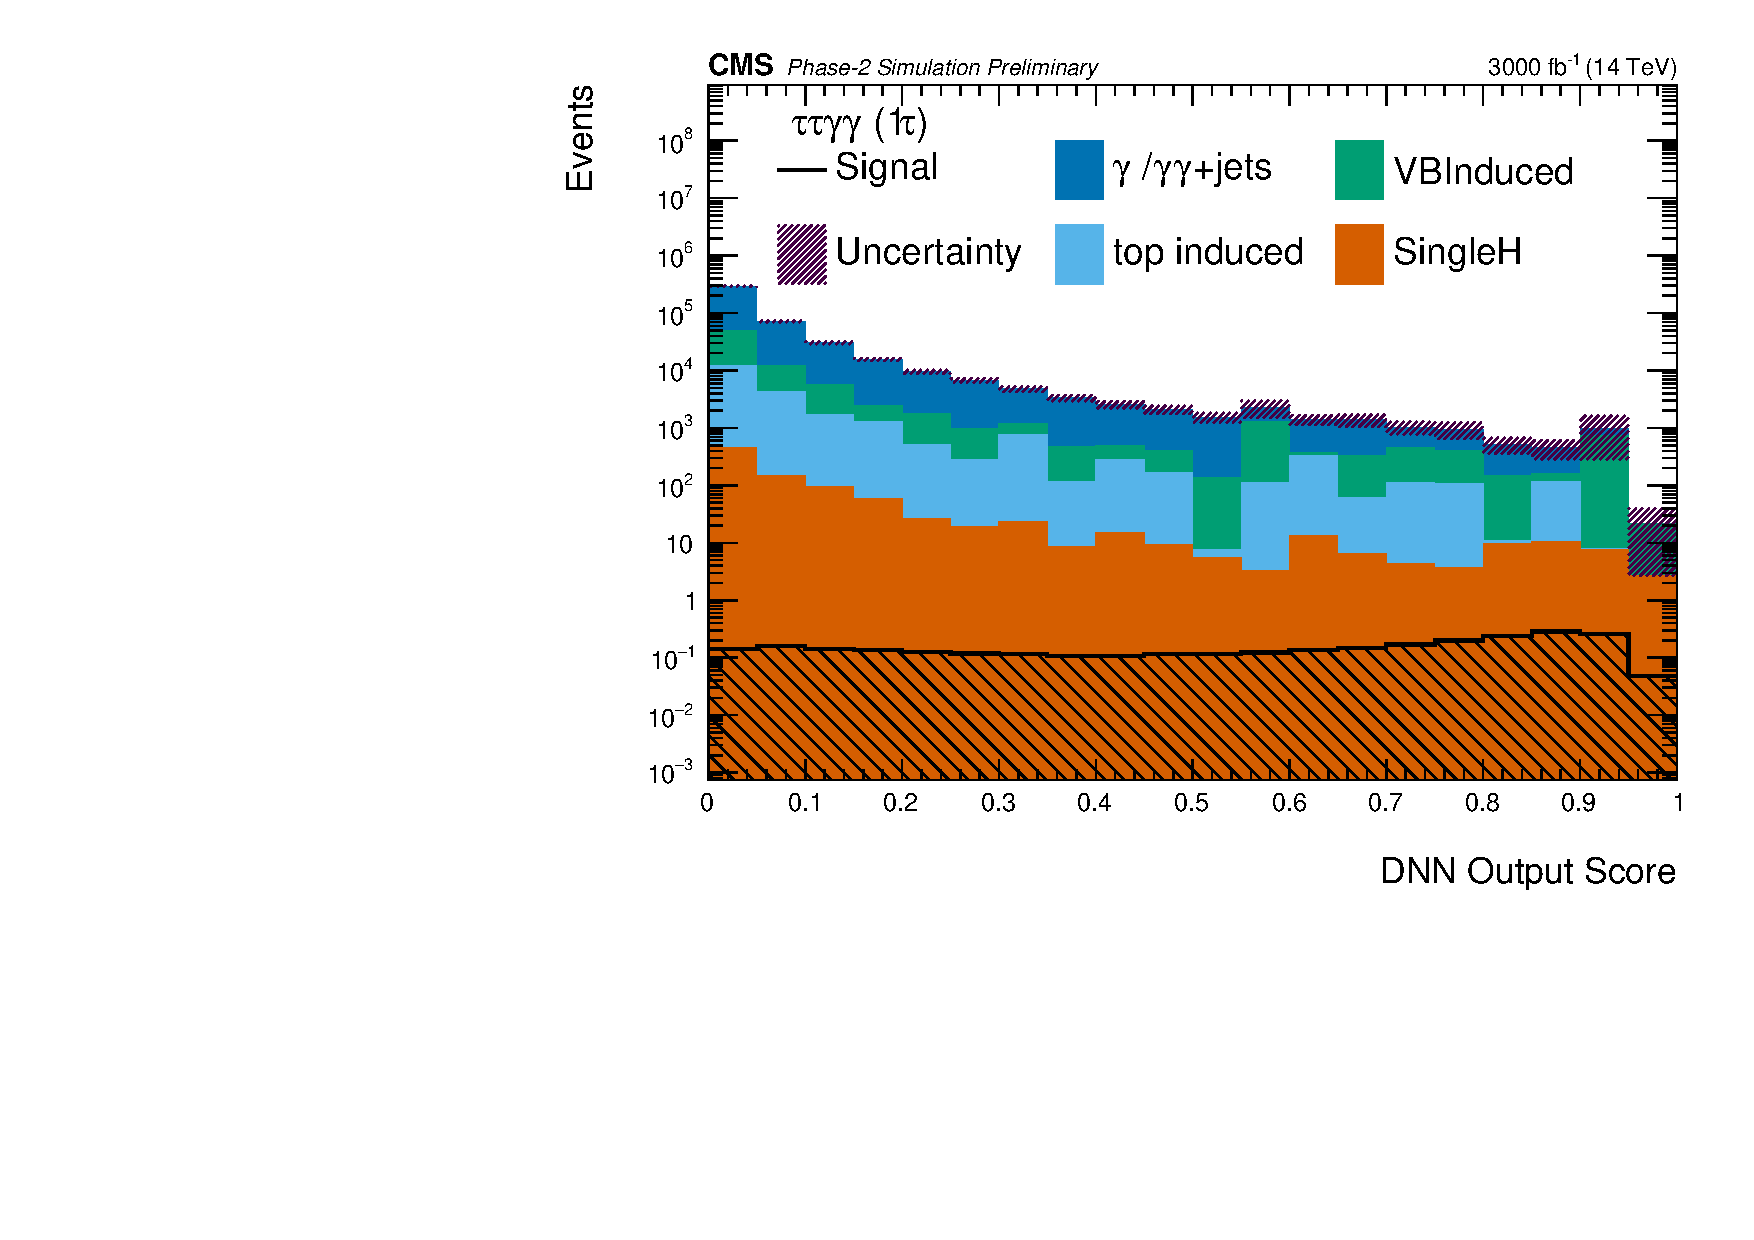
\includegraphics[width=0.75\textwidth]{Sections/Phase_II_HH/images/DNN/DNN_Score_tt_logy.pdf}
    \caption{One tau DNN output score distribution.}
    \label{fig:tau_perf}
\end{figure}

Events are partitioned into two categories based on the DNN score. Category one corresponds to events where the DNN score lies between 0.1 and 0.65, while events with a DNN score higher than 0.65 are placed into category 2. 




\subsection{Two Tau leptons final state}

Events fall into the two $\tau$ final state if they contain at least one diphoton candidate, at least two hadronically decaying taus, and zero electrons and photons. For the taus, it is required that they be oppositely charged because they are expected to come from a neutral Higgs boson. In this final state category, no additional selections are required. 
\section{Systematic uncertainties} \label{sec:Phase_II_Systematics}

The contribution of systematic uncertainties have been divided in experimental and theoretical uncertainties. Because the samples in this analysis are exclusively simulation based, experimental uncertainties are estimated from simulation. 
The experimental uncertainties are shown in Table \ref{tab:expUncertainties}, and follow the common Phase II projection uncertainties folloiwing the Yellow Report recommendation described in Ref.\cite{YRSystematics}. 
Theoretical uncertainties are added on the ggHH signal and single Higgs boson processes, as described in Table \ref{tab:ThUncertainties2}. 

\begin{table}[htb!]
  \centering
  \begin{tabular}{ll}
    \hline 
    Uncertainty Source & Input (\%) \\
    \hline
    Luminosity & 1 \\ 
    Diphoton trigger & 2 \\ 
    \mgg resolution & 5 \\ 
    PhotonID & 0.5/photon \\ 
    electronID & 0.5/electron \\
    muonID & 0.5/muon \\
    tauID & 2.5/tau\\
    Tau energy scale & 3 \\
    Jet energy Scale  & 3 \\
    b-tagging veto & 3 \\
    \hline
   \end{tabular}
    \caption{
    Experimental uncertainties considered in this study. 
    }
    \label{tab:expUncertainties}
\end{table}

\begin{table}[htb!]
  \centering
  \begin{tabular}{l|l|l|l}
    \hline 
    %\multicolumn{4}{c}{Theoretical uncertainties considered on ggHH signal yields}\\
    \hline
     Process & \multicolumn{3}{c}{Uncertainty Source} \\
    \hline
      & PDF $+ \alpha_s$ (\%) & QCD Scale (\%) & $m_{top}$ (\%)  \\
    \hline
    \hline
    ggHH & $\pm$ 3 & +2.1/-4.9 & +4.0/-18 \\
    \hline
    
    ggH & +4.6/-6.7 & $\pm$ 3.2 & - \\ 
    VBFH & +0.5/-0.3  & $\pm$ 2.1 & - \\
    VH & +0.4/-0.7  & $\pm$ 1.8 & - \\
    ttH & +6/-9.2  &  $\pm$ 3.5 & - \\
    tHq & +6.4/-14.7  & $\pm$ 3.6 & - \\ 

    \hline
  \end{tabular}
  \caption{
    Theoretical uncertainties considered on the ggHH signal and single Higgs processes.
  }
  \label{tab:ThUncertainties2}
\end{table}


\section{Results} \label{sec:Phase_II_results}

The expected Phase-2 \mgg distributions are shown in Figure~\ref{fig:prefit} for the semi-leptonic \wwgg final state, and one tau \ttgg final state. 

\begin{figure}[!htbp]
    \setcounter{subfigure}{0}
    \centering
    \subfloat[Semi-leptonic final state]{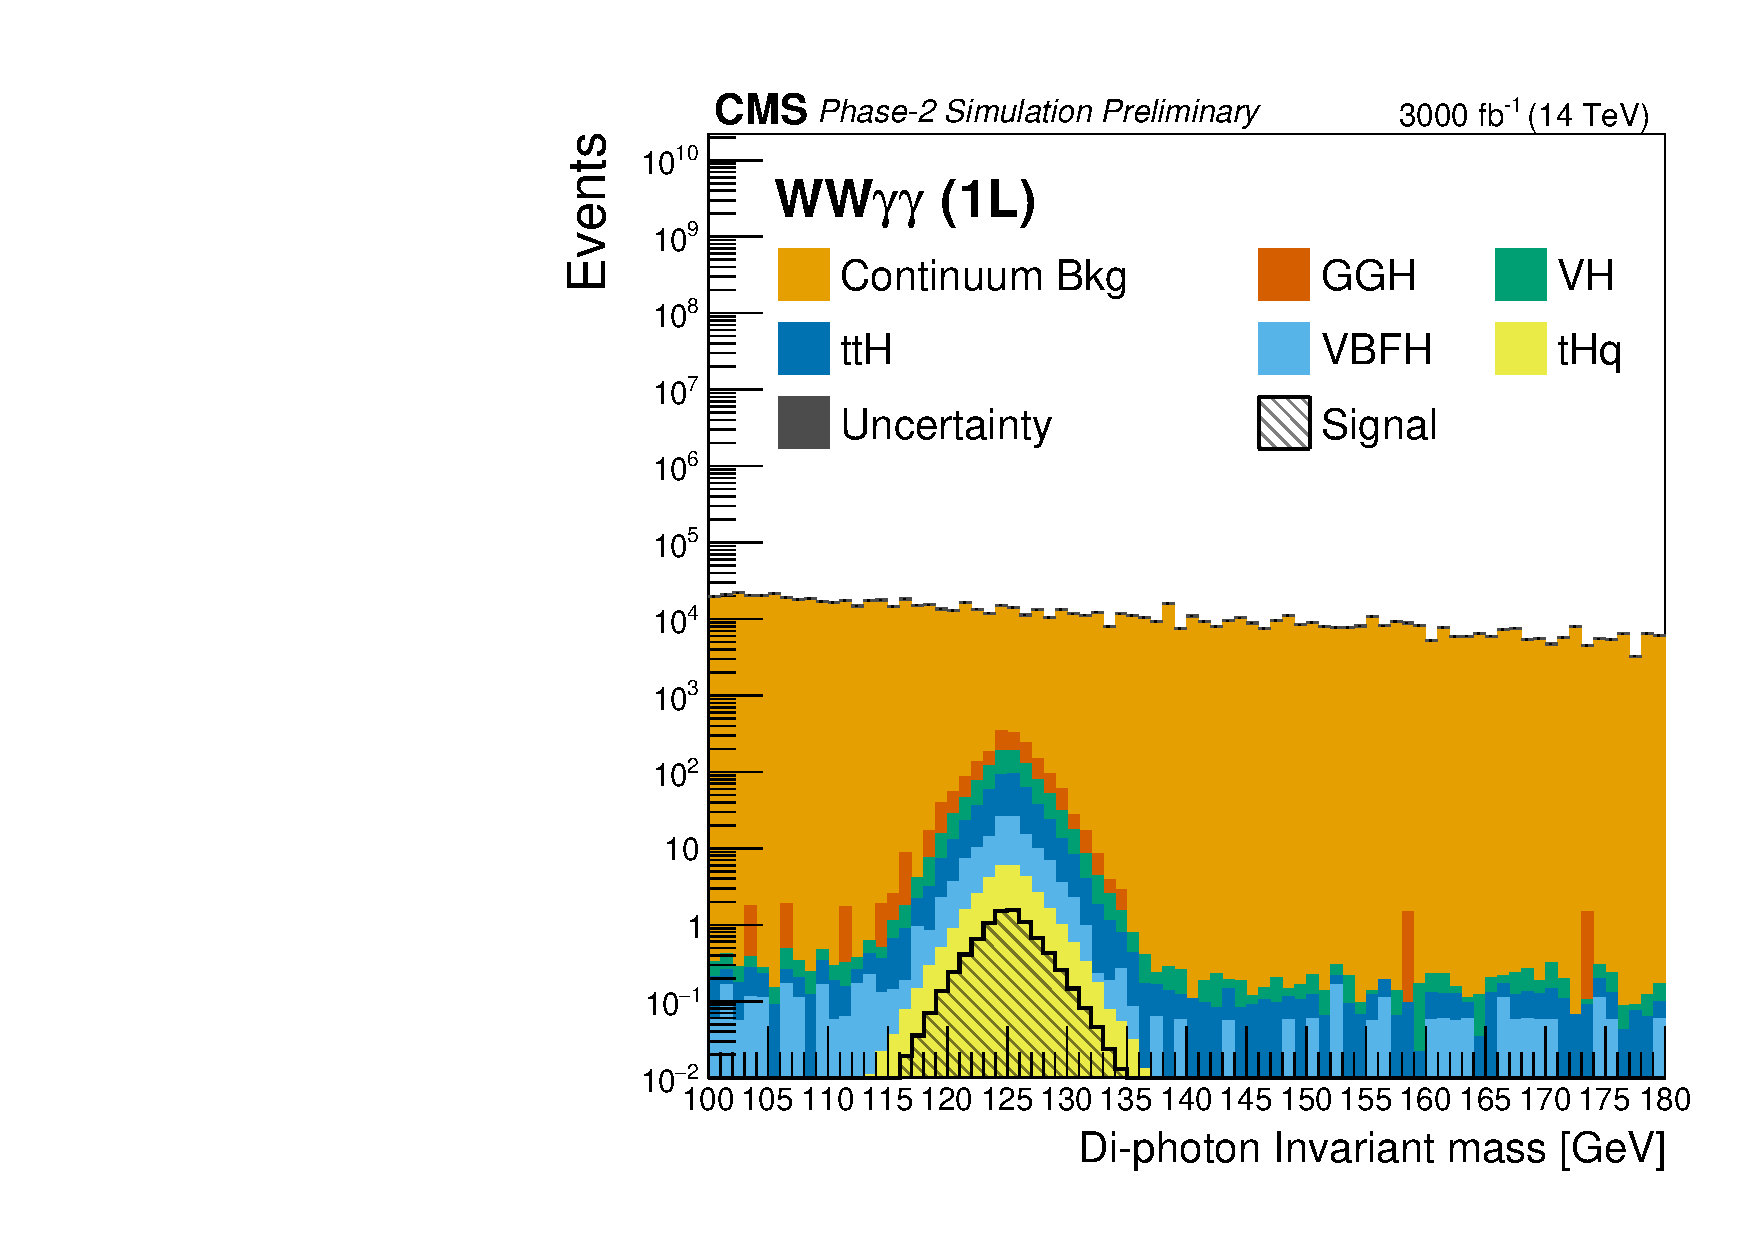
\includegraphics[width=0.45\textwidth]{Sections/Phase_II_HH/images/Results/CombineInputs/WWgg_1L_prefit_log_unblinded_False_HL.pdf}}
    \qquad
    \subfloat[One tau final state]{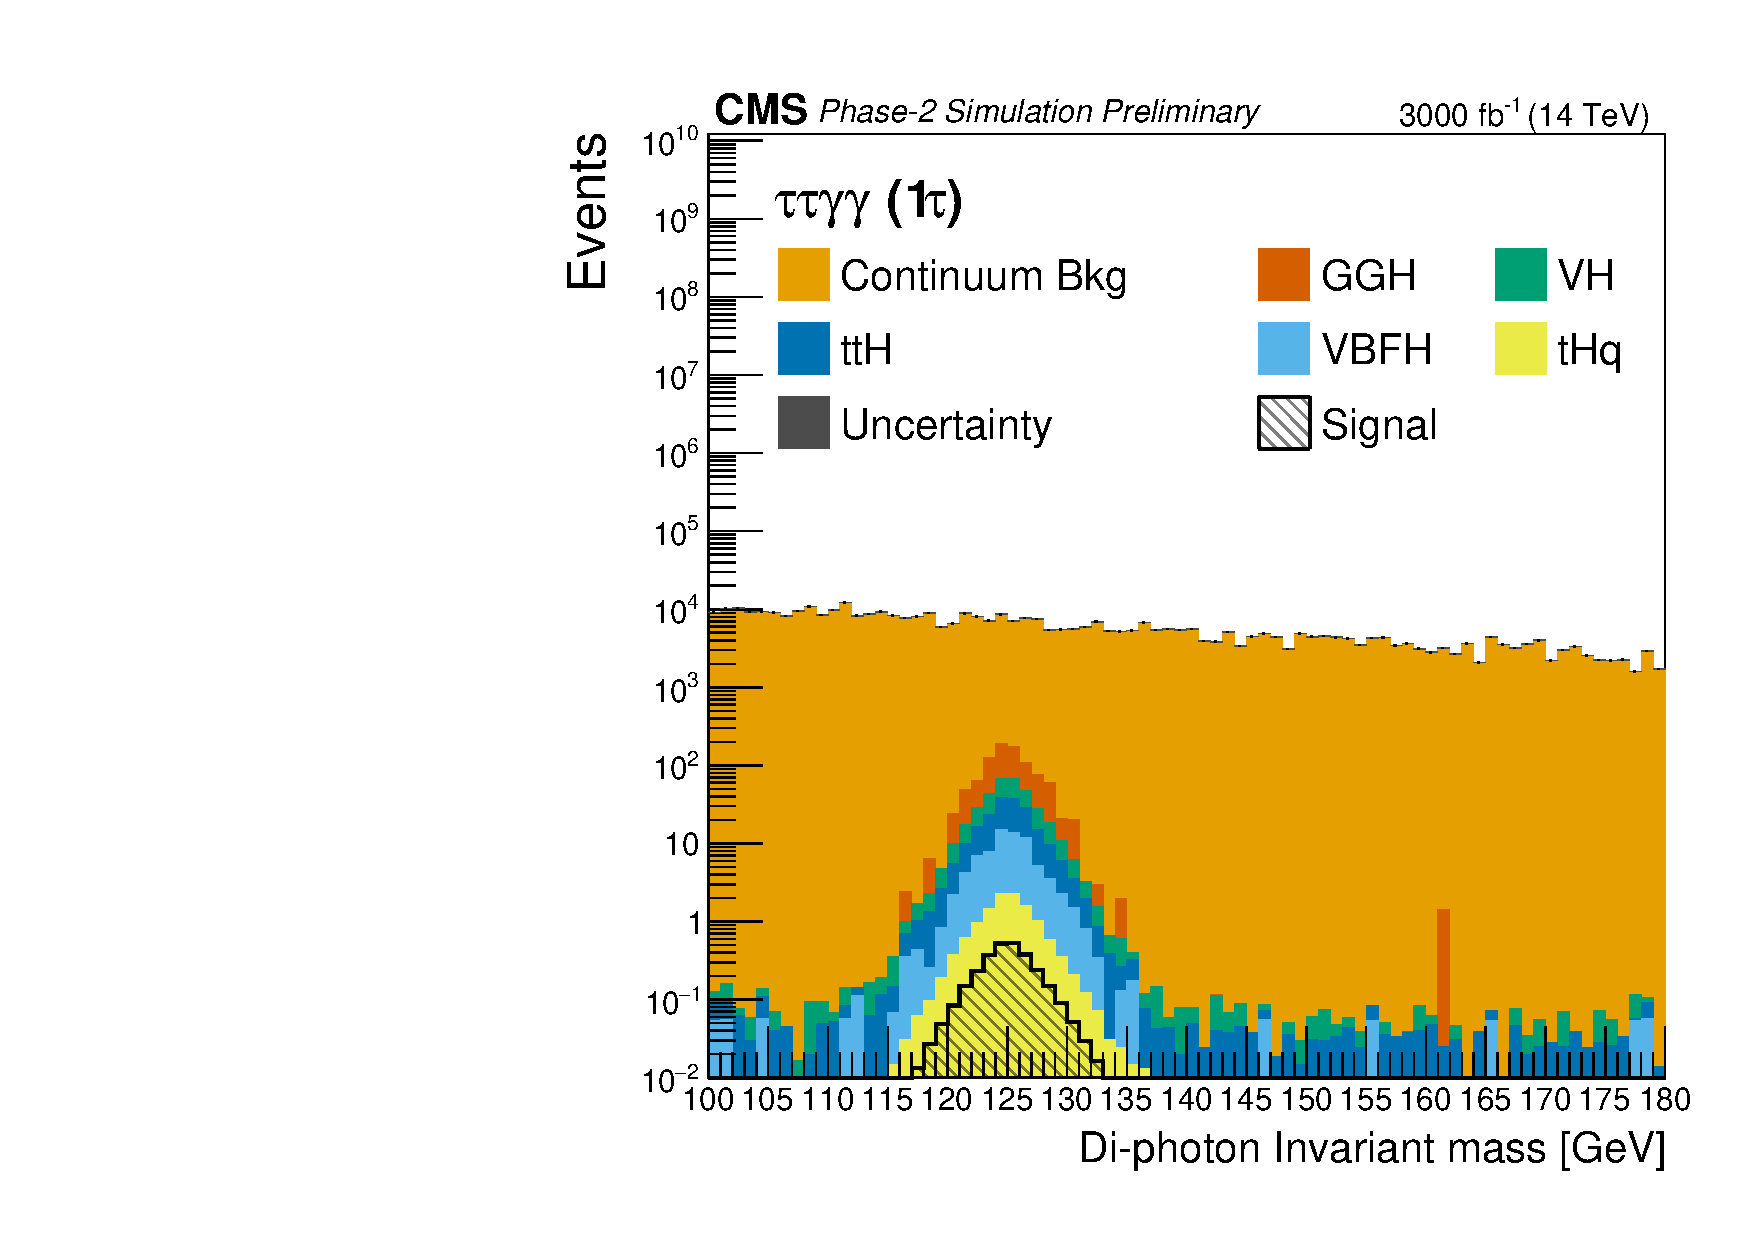
\includegraphics[width=0.45\textwidth]{Sections/Phase_II_HH/images/Results/CombineInputs/ttgg_prefit_log_unblinded_False_HL.pdf}}
    \caption{$m_{\gamma\gamma}$ distributions in the \wwgg, Semi-leptonic (left) and \ttgg, 1$\tau$ (right) final states.}
    \label{fig:prefit}
\end{figure}

Given the presence of high fluctuations in the \mgg distribution of the continuum background across different categories, a falling exponential function is fit to the continuum background templates and used as the final background template for each category. After applying this exponential fit, and a gaussian fit to each HH and H template, the diphoton invariant mass distributions for the Semi-leptonic final state in its most sensitive category, the single fully-leptonic category and in the single 2 $\tau$ final state category are shown in Figure \ref{fig:final_plots}, where signal HH and single Higgs templates are modelled as Gaussian functions fit to the diphoton mass distributions, and the continuum background is modelled by exponential functions. The (pseudo-)data are generated according to the fitted signal, single Higgs and continuum background contributions.  

\begin{figure}[!htbp]
    \setcounter{subfigure}{0}
    \centering
    \subfloat[Semi-leptonic final state, Category 4]{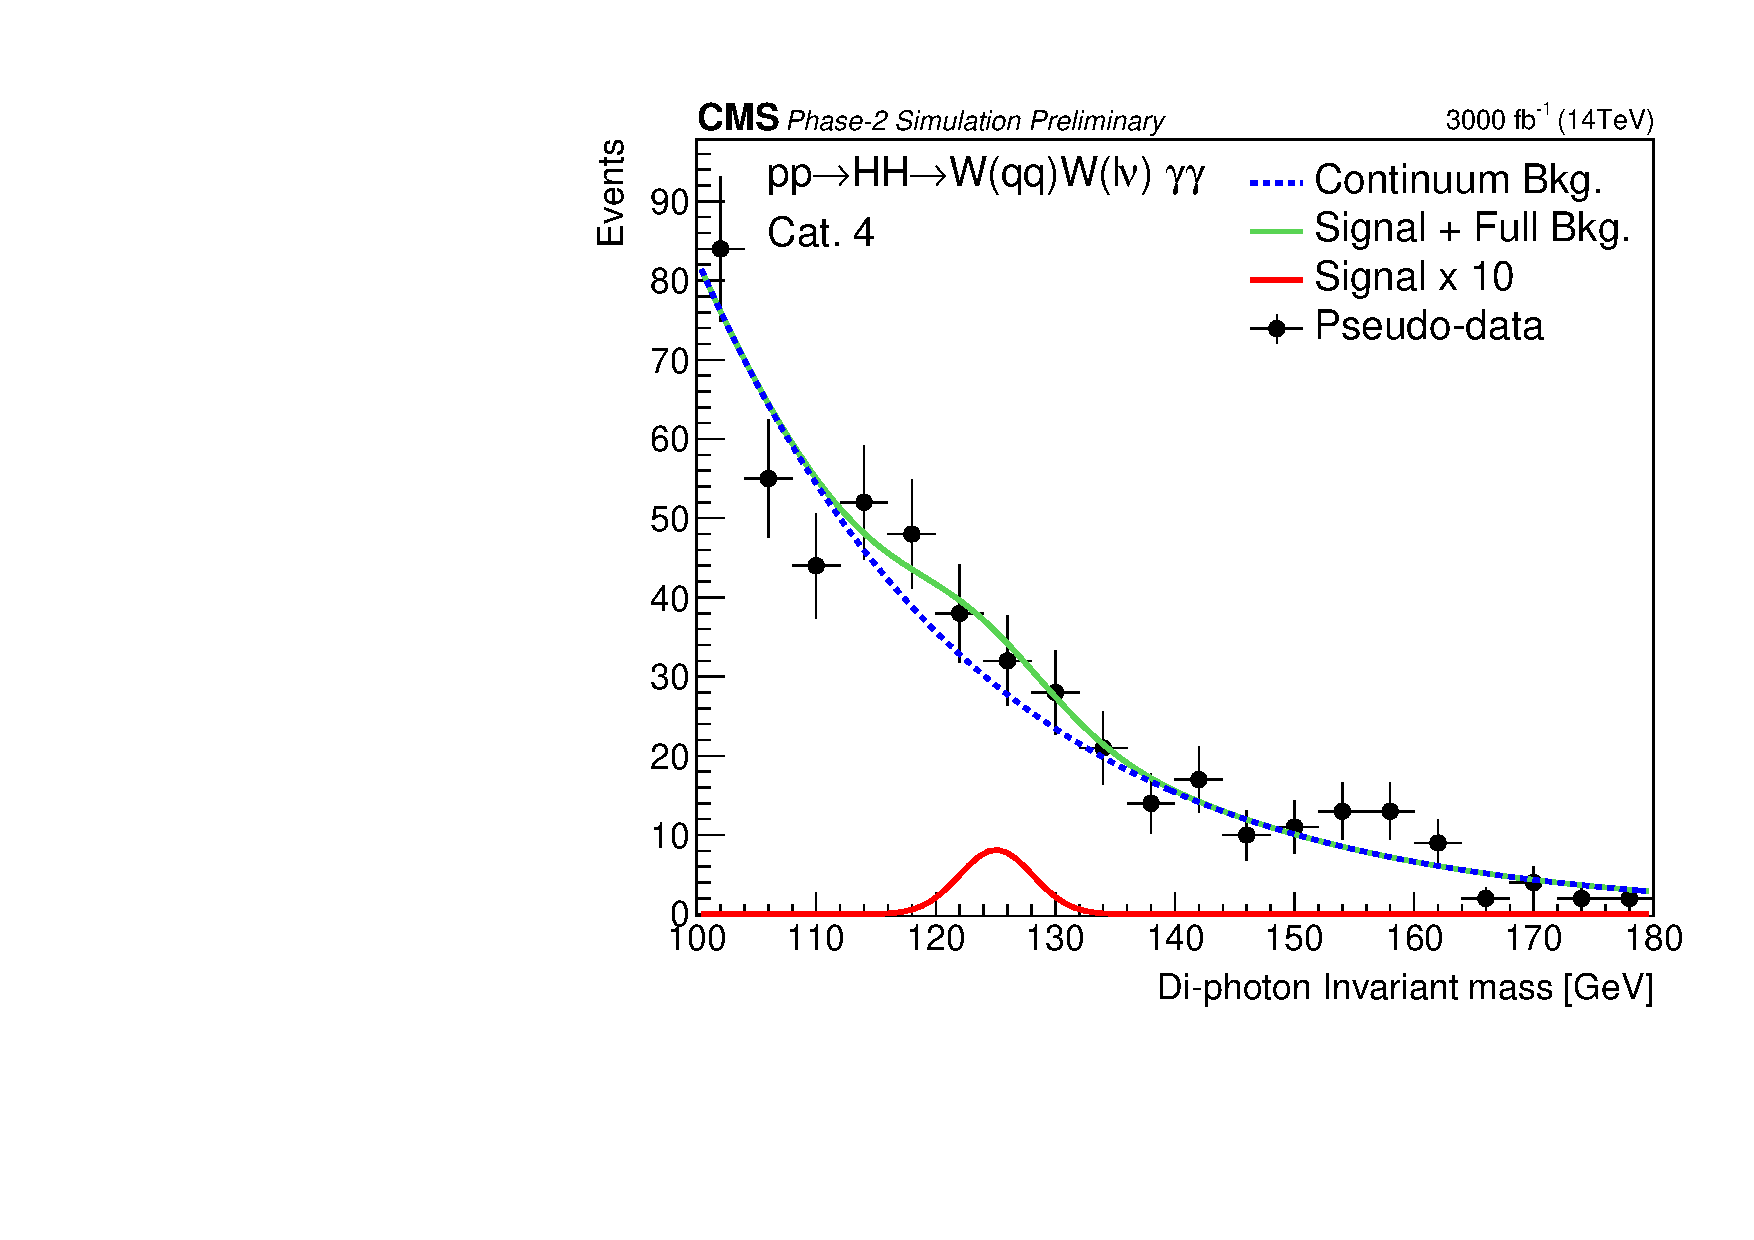
\includegraphics[width=0.45\textwidth]{Sections/Phase_II_HH/images/Results/Inv_mass_gghasOneL_DNN_4_HL_FIT.pdf}}
    \qquad
    \subfloat[Fully-leptonic final state]{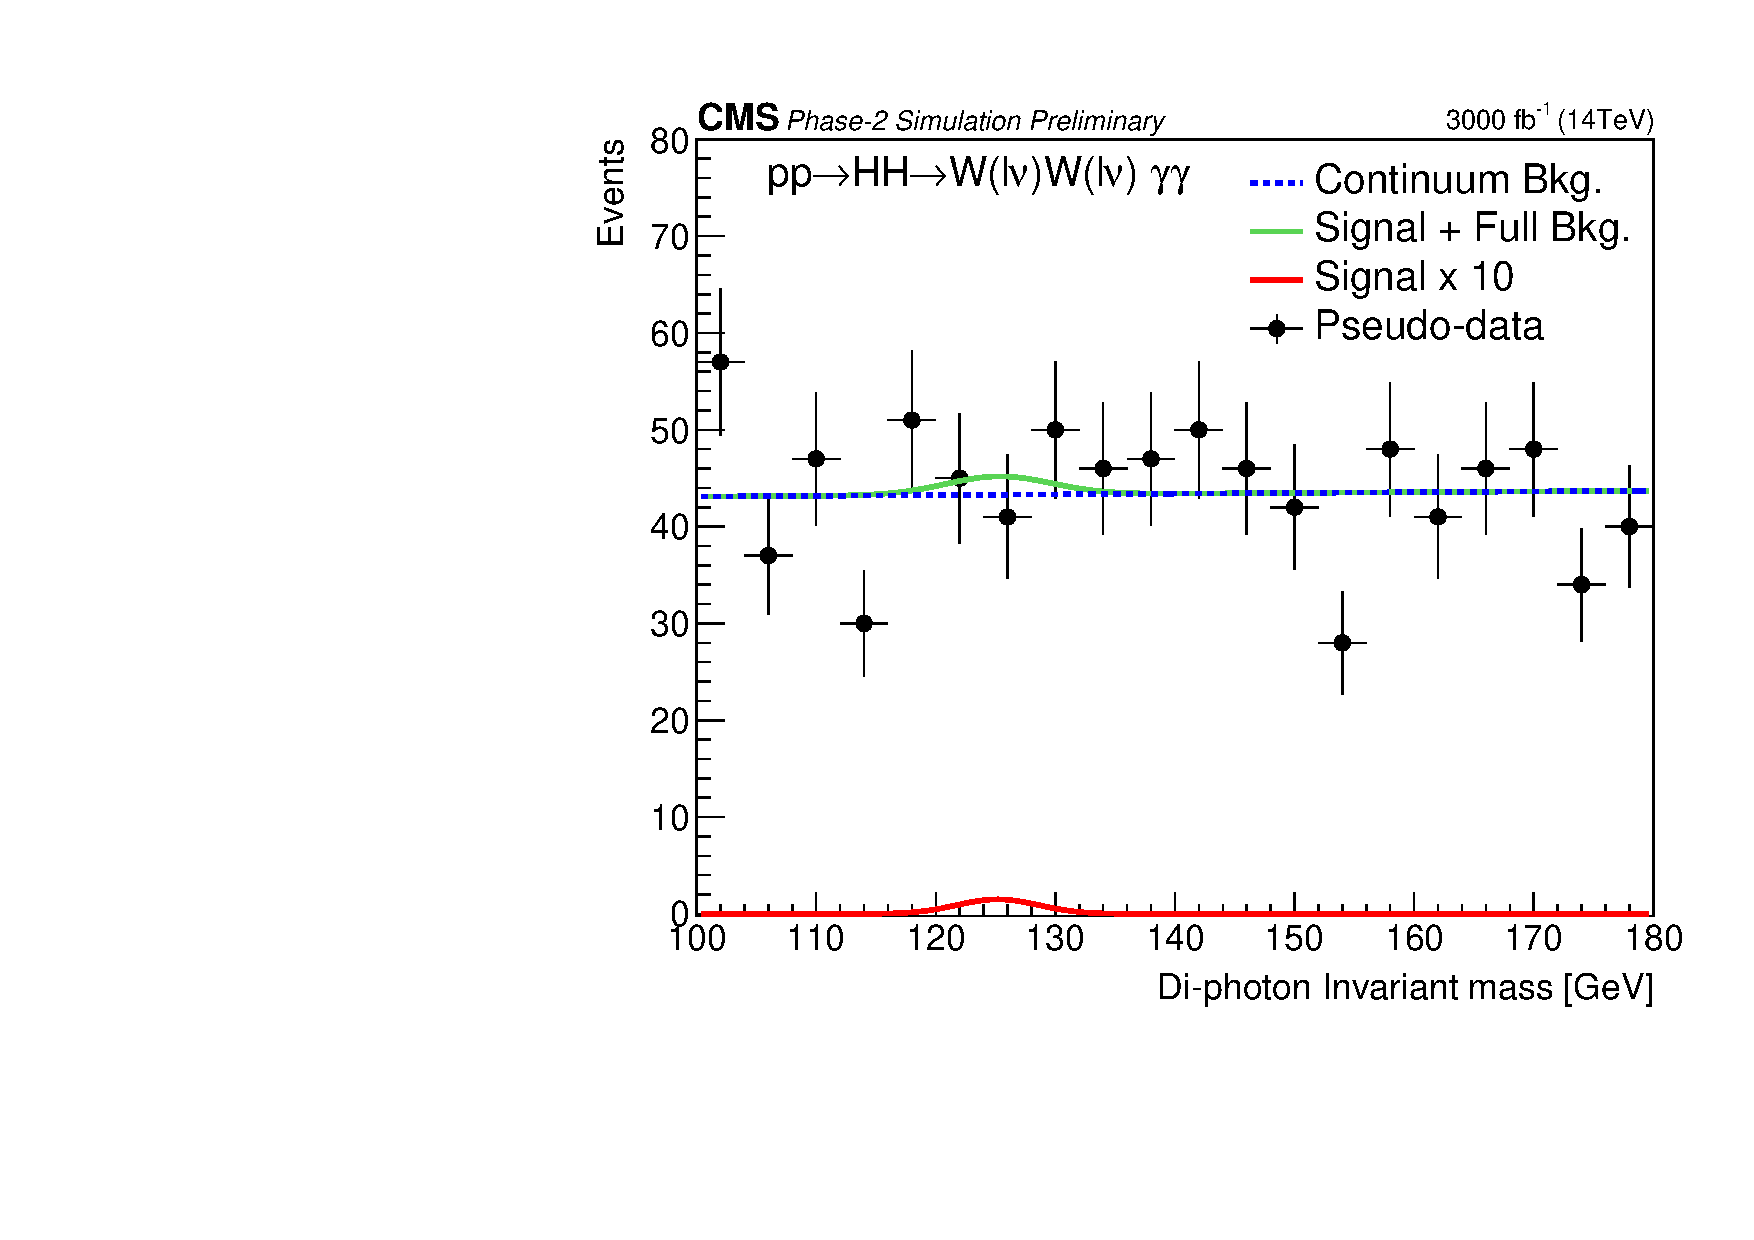
\includegraphics[width=0.45\textwidth]{Sections/Phase_II_HH/images/Results/Inv_mass_gghasTwoL_HL_FIT.pdf}}
    \qquad
    \subfloat[Two taus final state]{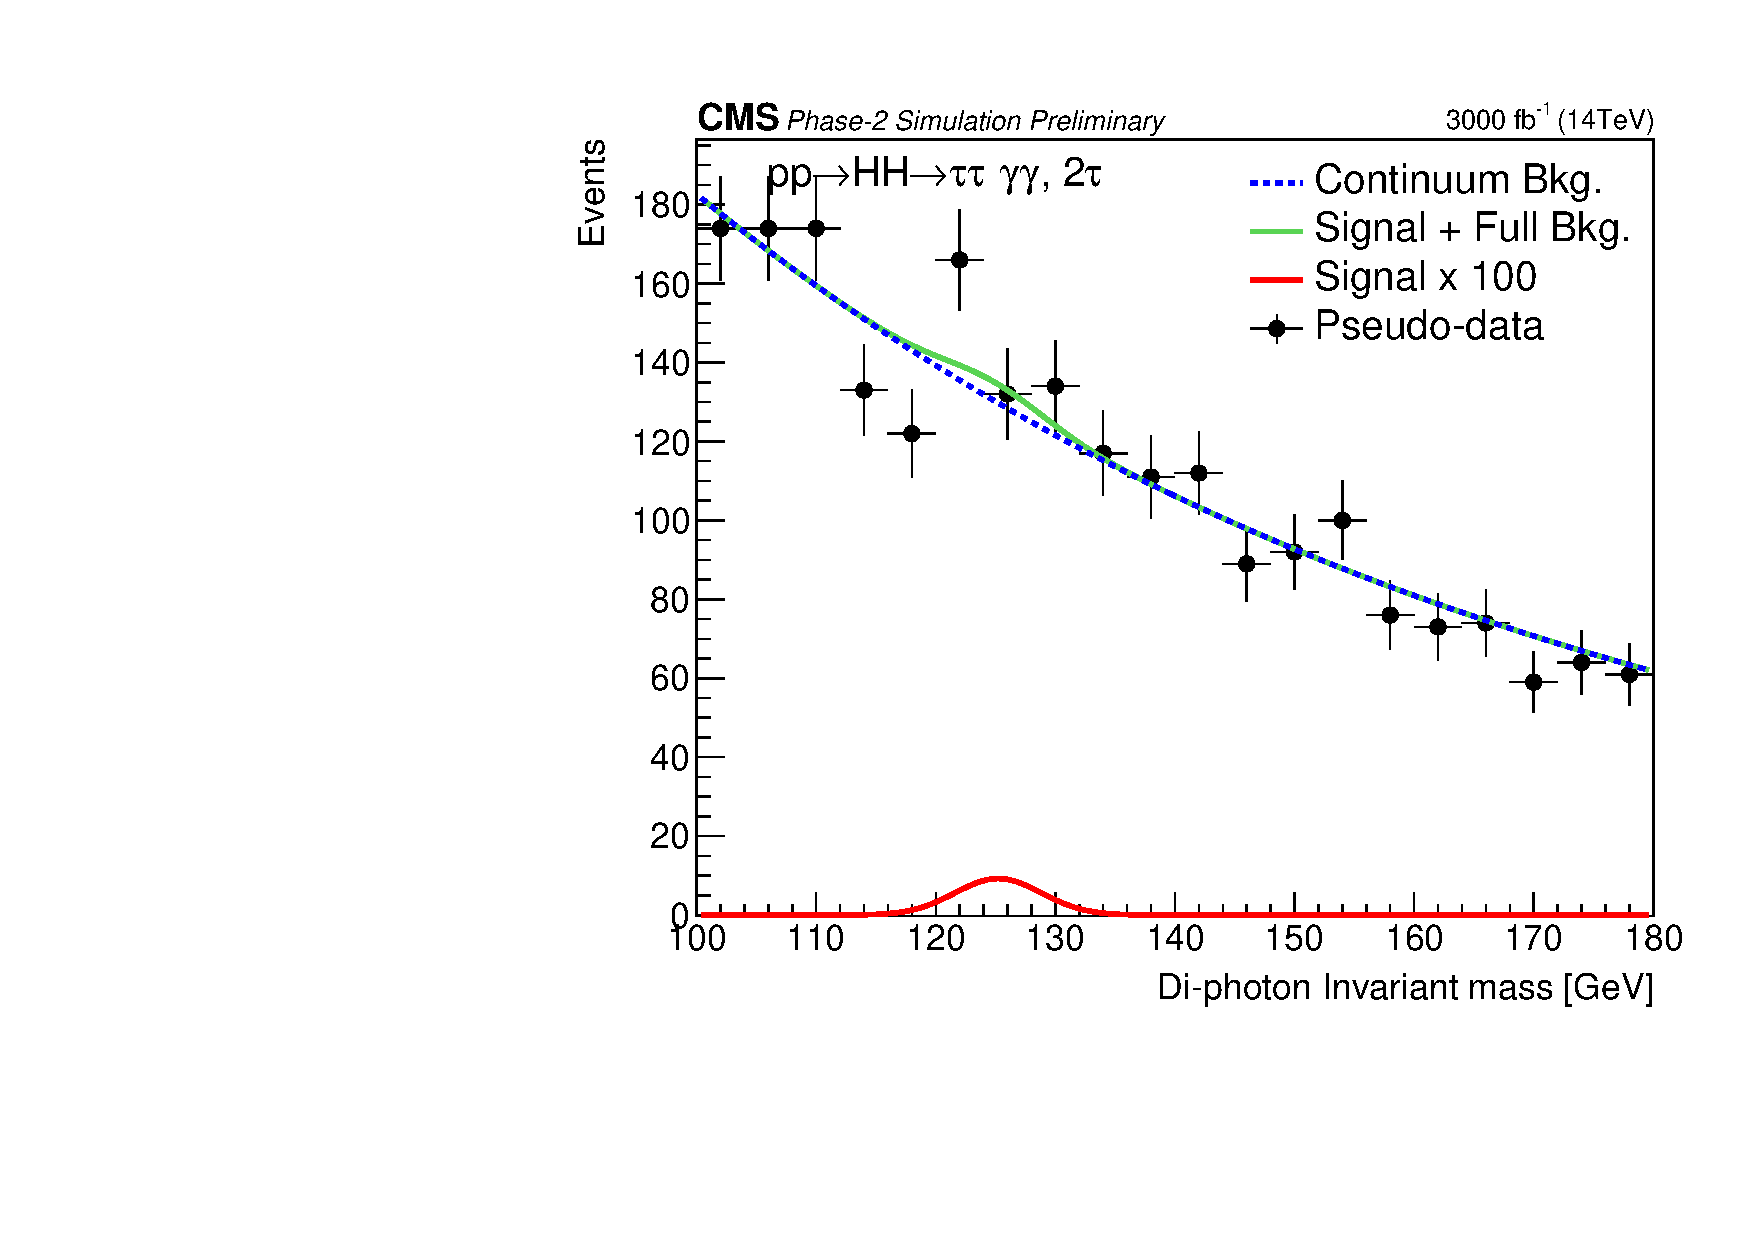
\includegraphics[width=0.45\textwidth]{Sections/Phase_II_HH/images/Results/Mgg_c4_Zveto_HL_FIT.pdf}}
    \caption{$m_{\gamma\gamma}$ distributions in the \wwgg, Semi-leptonic (top left), Fully-leptonic (top right) and \ttgg, 2$\tau$s (bottom) final states.}
    \label{fig:final_plots}
\end{figure}

The expected signal significance is extracted by fitting the background-only \mgg template to the signal $+$ background template simultaneously in all categories, following a binned maximum likelihood
approach, with all systematic uncertainties treated as nuisance parameters with log-normal distributions. The correlations among different sources of uncertainties are taken into account while the different final states are considered as independent channels in the fit. 

The significance values obtained are shown in Table~\ref{tab:combinedSignificance} for the WW$\gamma\gamma$ and \ttgg final states along with their combination.

\begin{table}[h!]
  \centering
  \begin{tabular}{lc}
    \hline 
    Final State & Significance (stat+exp+theory) \\
\hline

    \wwgg & 0.21  \\ 
    \ttgg &  0.08 \\
   Combination &  0.22 \\ 

    \hline
   \end{tabular}
    \caption{
        Expected HL-LHC significances ($\sigma$) results of the WW$\gamma\gamma$ and \ttgg processes with their combination.
        }
    \label{tab:combinedSignificance}
\end{table}

A combined significance of 0.22$\sigma$ is extracted, combining the \wwgg and \ttgg categories. 
\section{Summary} \label{sec:Phase_II_Summary}

A projection of the sensitivity of non-resonant Higgs boson pair production in the WW$\gamma\gamma$ and \ttgg final states has been performed, using simulated proton-proton collision events at a center-of-mass energy of 14 TeV and integrated luminosity of 3000 fb$^{-1}$ at the future HL-LHC. Additionally, the response of the future Phase II CMS detector has been simulated. For the \wwgg and one tau \ttgg final states of this analysis, the analysis strategy and techniques from the Run 2 \wwgg analysis are used. 

Combining all final state categories and including systematic uncertainties, a combined expected significance of $0.22$ $\sigma$ is measured.

When considering a projection analysis, it is important consider a few caveats to the result. The first is that because the analysis is simulation only, it is not possible to make the use of data-driven techniques, such as the one used for the Fully-hadronic final state of the Run 2 \wwgg analysis. Additionally, as the HL-LHC and Phase II CMS detector have not yet been assembled, physicists have not yet had a chance to study this new detector's response to new data-taking conditions. Such studies can often include the optimization of the detector's ability to identify particles, and thus can lead to improved identification and analysis sensitivity. 

